\section{Literature Review}
\label{sec:related_work}

\subsection{Self-supervised Representation Learning}
\subsubsection{SimCLR: Simple Framework for Contrastive Learning of Visual Representations}
SimCLR\cite{chen2020simple} is a contrastive self-supervised learning framework that learns visual representations of images without requiring labeled data. The paper explores various components of the model and showcases the importance of each component via numbers from experiments.

The first key component of the SimCLR model is the augmentations it applies, which lead to the positive and negative pairs needed to perform contrastive learning. The mentioned model stochastically chooses two augmentations from the chosen three augmentations to get the training pairs. The paper also mentions various other augmentations but reinforces the choice of the three augmentations (random crop, random colorization, and random Gaussian noise).

\begin{figure}[h]
\small
    \centering
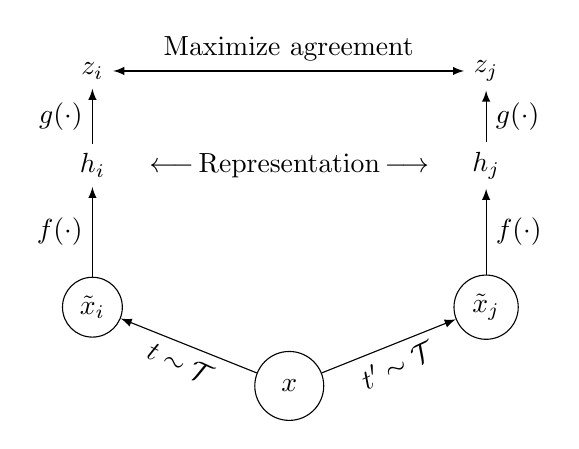
\begin{tikzpicture}
    \node at (0,1.8) (h) {$\longleftarrow\,$Representation$\,\longrightarrow$};
    \node[draw, circle] at (0,-1) (x) {$\,~\bm{x}~\,$};
    \node[draw, circle] at (-2.5,0) (x1) {$\tilde{\bm{x}}_i$};
    \node[draw, circle] at (2.5,0) (x2) {$\tilde{\bm{x}}_j$};
    \node at (-2.5,1.8) (h) {$\bm h_i$};
    \node at (2.5,1.8) (c) {$\bm h_j$};
    \node at (-2.5,3) (hh) {$\bm z_i$};
    \node at (2.5,3) (cc) {$\bm z_j$};
    \path[->] 
        (x)  edge [>=latex] node[below,rotate=-25] {$t\sim\mathcal{T}$} (x1)
        (x)  edge [>=latex] node[below,rotate=25] {$t'\sim \mathcal{T}$} (x2)
        (x1)  edge [>=latex] node[left,rotate=0] {$f(\cdot)$} (h)
        (x2)  edge [>=latex] node[right,rotate=0] {$f(\cdot)$} (c)
        (h)  edge [>=latex] node[left,rotate=0] {$g(\cdot)$} (hh)
        (c)  edge [>=latex] node[right,rotate=0] {$g(\cdot)$} (cc);
    \path[<->]
        (hh)  edge [>=latex] node[above,rotate=0] {Maximize agreement} (cc);
    \end{tikzpicture}
    \caption{A simple framework for contrastive learning of visual representations. 
    Two separate data augmentation operators are sampled from the same family of augmentations ($t\sim \mathcal{T}$ and $t'\sim \mathcal{T}$) and applied to each data example to obtain two correlated views.
    A base encoder network $f(\cdot)$ and a projection head $g(\cdot)$ are trained to maximize agreement using a contrastive loss. After training is completed, we throw away the projection head $g(\cdot)$ and use encoder $f(\cdot)$ and representation $\bm h$ for downstream tasks.}
    \label{fig:framework}
\end{figure}

Batches of such augmented images are fed to the encoder component where a ResNet architecture was used. The paper then experimented with different projection layers and showed via experimentation that a non-linear projection component worked the best. The contrastive loss is then applied to these projected outputs. SimCLR shows various key components that can be used to extract representations in a self-supervised manner which can be made use of to come up with an explainable self-supervised learning model.

\subsubsection{Learning features by Swapping Assignments between multiple Views (SwAV) of an Image}
SwAV (Swapping Assignments Between Views) \cite{caron2020unsupervised} is a self-supervised learning method that introduces a clustering-based approach to learning visual representations without explicit contrastive loss. SwAV directly learns cluster assignments for different augmentations of the same image. This is achieved by using a swapped prediction mechanism, where the model predicts the cluster assignment of one view using the features of another as seen in the loss function:
\begin{eqnarray}
L(\mathbf{z}_t, \mathbf{z}_s) & = &\ell(\mathbf{z}_t, \mathbf{q}_s) + \ell(\mathbf{z}_s, \mathbf{q}_t),
\label{eq:twoviews}
\end{eqnarray}

The terms in the loss function representing the swapped prediction terms are defined as the cross-entropy loss between the code and the probability obtained by taking a softmax of the dot products of ${z_i}$ and all prototypes in C (set of learned prototypes). Some improvements that the SwAV paper proposes firstly is computing the codes in an online fashion and secondly is the choice of another image augmentation, namely Multi-crop. In the multi-crop strategy we use two standard resolution crops and sample additional low resolution crops that cover only small parts of the image because comparing random crops of an image plays a central role by capturing information in terms of relations between parts of a scene or an object.

\begin{figure}[t]
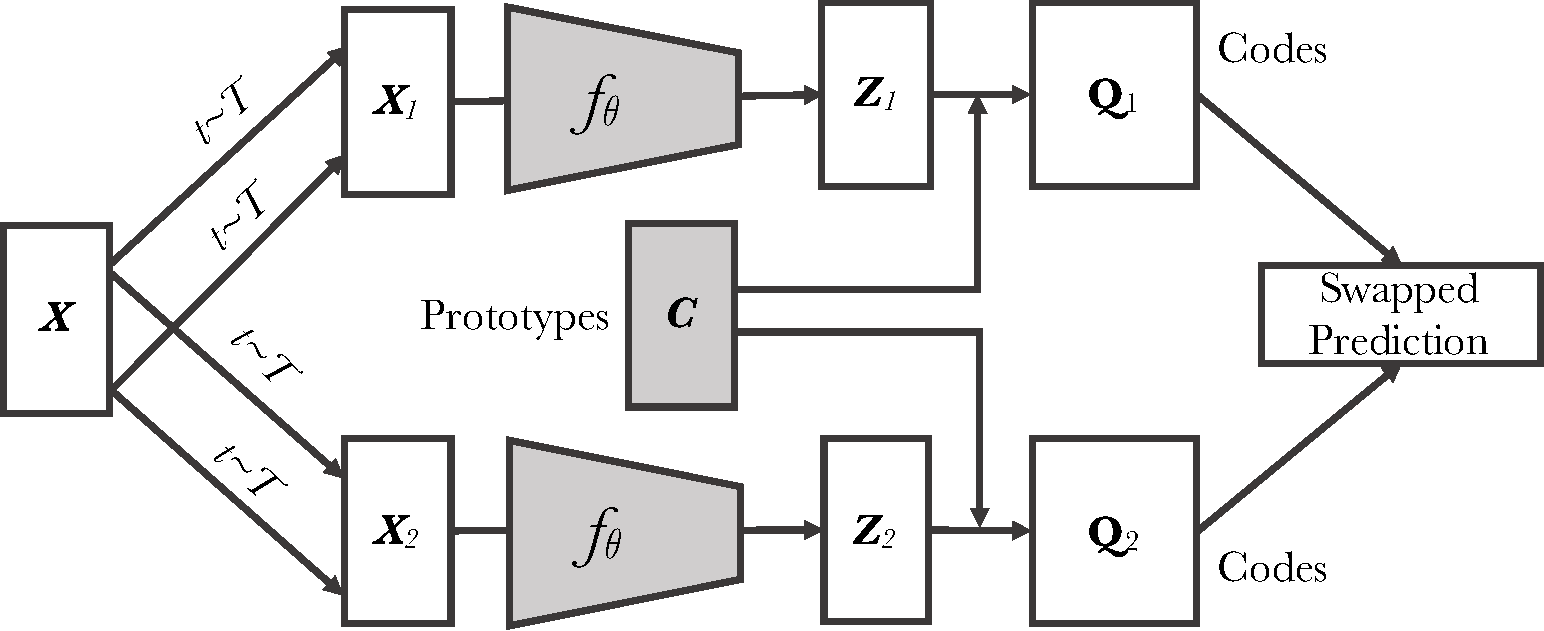
\includegraphics[height=.4\linewidth]{images/oto_simple.pdf}
\caption{
We first obtain ``codes'' by assigning features to prototype vectors.
We then solve a ``swapped'' prediction problem wherein the codes obtained from one data augmented view are predicted using the other view.
Prototype vectors are learned along with the ConvNet parameters by backpropragation. 
}
\end{figure}

\subsubsection{MoCo: Momentum Contrast for Unsupervised Visual Representation Learning}
Momentum Contrast (MoCo) \cite{he2020momentum} is a self-supervised learning framework built on the idea of contrastive learning. MoCo maintains a dynamic dictionary of negative samples using a momentum-based encoder. This dictionary is implemented as a queue, where old representations are progressively replaced by new ones. The novelty that MoCo introduces in its momentum encoder, which helps maintain consistency in feature representations over time and reduces memory constraints by allowing the model to use a relatively smaller batch size while still accessing a large pool of negative samples.

\begin{figure}[t]\centering
\vspace{1.em}
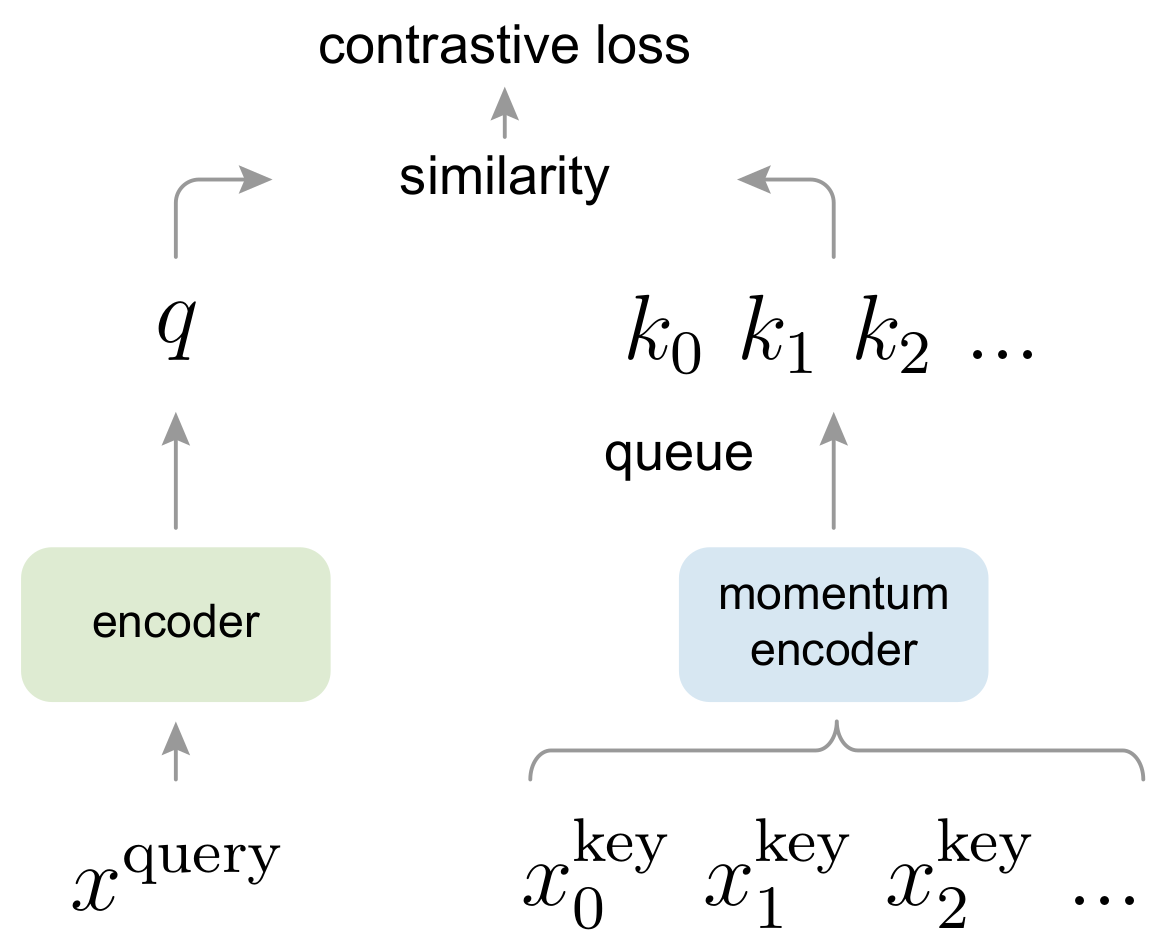
\includegraphics[width=.65\linewidth]{images/MoCo_Architecture.png}
\caption{Momentum Contrast (MoCo) trains a visual representation encoder by matching an encoded query $q$ to a dictionary of encoded keys using a contrastive loss. The dictionary keys $\{k_0, k_1, k_2, ...\}$ are defined on-the-fly by a set of data samples.
The dictionary is built as a queue, with the current mini-batch enqueued and the oldest mini-batch dequeued, decoupling it from the mini-batch size.
The keys are encoded by a slowly progressing encoder, driven by a momentum update with the query encoder.
This method enables a large and consistent dictionary for learning visual representations.
\label{fig:teaser}}
\vspace{-1em}
\end{figure}

The MoCo architecture consists of two encoders: a query encoder and a key encoder. The query encoder is updated via backpropagation, while the key encoder is updated using an exponential moving average (momentum update) to ensure stability as follows:
\begin{equation}
\theta_\textrm{k} \leftarrow m \theta_\textrm{k} + (1 - m) \theta_\textrm{q}.
\label{eq:moco}
\end{equation}
Given an image, two different augmentations are applied, producing a query image and a key image. The query image is encoded using the query encoder, and the key image is encoded using the momentum encoder. The contrastive loss, typically InfoNCE defined as follows:
\begin{equation}
\mathcal{L}_q = -\log \frac{\exp(q{\cdot}k_+ / \tau)}{\sum_{i=0}^{K}\exp(q{\cdot}k_i  / \tau)}
\label{eq:infonce}
\end{equation}
This loss is then applied to maximize similarity between the query and key embeddings while minimizing similarity with a queue of negative samples. This framework has been widely adopted in self-supervised learning due to its efficiency in handling large-scale datasets with limited computational resources.

\subsection{Explanibility Techniques}
\subsubsection{Grad-CAM: Visual Explanations from Deep Networks via Gradient-based Localization}

Gradient-weighted Class Activation Mapping (Grad-CAM)\cite{Selvaraju_2017_ICCV} is a widely adopted method that provides visual explanations for model predictions by leveraging gradient information to highlight the most important regions in an input image. Unlike earlier Class Activation Mapping (CAM) approaches, which required model modifications, Grad-CAM is architecture-agnostic and can be applied to various types of model architectures.

Grad-CAM generates class-specific saliency maps by computing the importance of feature maps in a CNN for a given target class. The method consists of the following steps:

1. \textbf{Forward Pass:} The input image is processed through the CNN, and feature maps \(A^k\) from a selected convolutional layer are extracted.

2. \textbf{Gradient Computation:} The gradients of the target class score \(y^c\) are computed with respect to each feature map:

   $$
   \alpha_k^c = \frac{1}{Z} \sum_i \sum_j \frac{\partial y^c}{\partial A^k_{ij}}
   $$

   where \(Z\) represents the spatial dimensions of the feature map.

3. \textbf{Weighted Feature Map Combination:} A weighted sum of the feature maps is computed using the importance weights \(\alpha_k^c\):

   $$
   L_c = \text{ReLU} \left( \sum_k \alpha_k^c A^k \right)
   $$

   The ReLU function ensures that only positive influences contribute to the visualization, preventing the inclusion of irrelevant or misleading features.

4. \textbf{Heatmap Generation and Overlay:} The resulting saliency map is re-sampled to the original image resolution and overlayed on the input image to highlight the key regions that contribute to the model decision.

\begin{figure}[h]
    \centering
    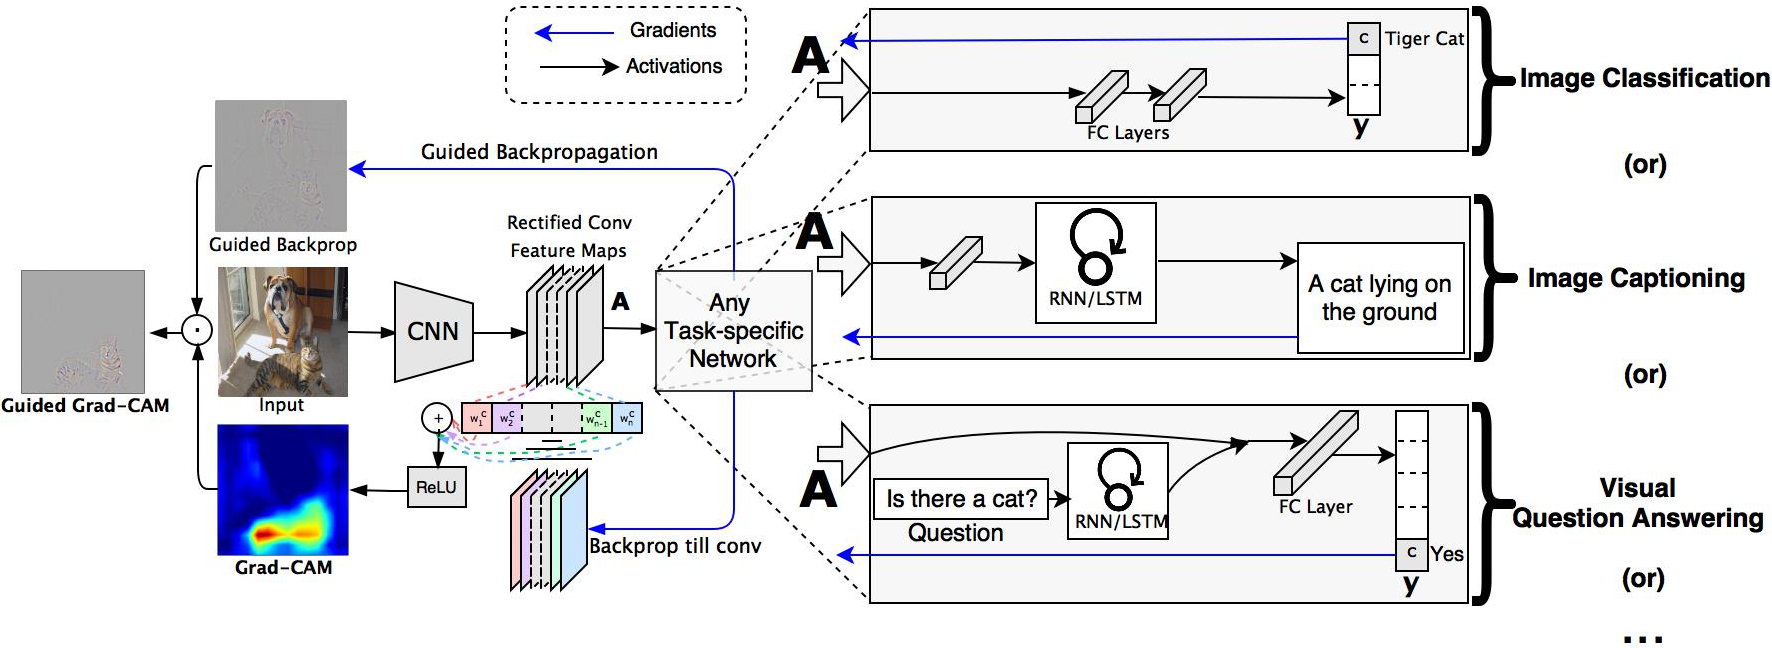
\includegraphics[width=0.47\textwidth]{./images/Grad-CAM_approach.png}
    \caption{Grad-CAM visualization of a ResNet-50 model for the class "zebra." The heatmap highlights the regions in the input image that are most relevant for the model's prediction.}
    \label{fig:gradcam}
\end{figure}

\subsubsection{RELAX: Representation Learning Explainability}
\begin{itemize}
    \item Representation Learning Explainability (RELAX)\cite{chen2020simple} is a novel framework for explaining representations that also quantify their uncertainty.
    \item It measures the change in the representation of an image when compared with the masked version of the image.
    \item The central idea is that when informative parts are masked out, the representation should change significantly, i.e., the similarity between masked and unmasked representations should be low when informative parts are masked out and high when uninformative parts are masked out.
\end{itemize} 
Let $\mathbf{X}\in \mathbb{R}^{H\times W}$ represents image of dimensions $H\times W$ and $f$ be the feature extraction model that extracts representation $\mathbf{h} = f(\mathbf{X}) \in \mathbb{R}^D$. \\
To create masked images, we apply a stochastic mask $\mathbf{M}\in [0, 1]^{H\times W}$, where $M_{ij}$ is drawn from some distribution.
The masked representation is given by $\bar{\mathbf{h}} = f(\mathbf{X}\odot \mathbf{M})$, where $\odot$ denotes element-wise multiplication.\\
The similarity between masked and unmasked representations is measured using cosine similarity, 
\begin{equation*}\label{eq:sim}
    s(\mathbf{h}, \bar{\mathbf{h}}) = \frac{\langle \mathbf{h}, \bar{\mathbf{h}}\rangle }{\lVert\mathbf{h}\rVert \lVert\bar{\mathbf{h}}\rVert},
\end{equation*}, where $\lVert\cdot\rVert$ denotes the Euclidean norm of a vector. \\
Importance $R_{ij}$ of pixel $(i,j)$ is defined as:
\begin{equation*}\label{eq:rel1}
    R_{ij} = \mathrm{E}_{\mathbf{M}}\big[s(\mathbf{h}, \bar{\mathbf{h}})M_{ij}\big].
\end{equation*}
\begin{equation*}\label{eq:rel2}
    \bar{R}_{ij} = \frac{1}{N}\sum\limits_{n=1}^N s(\mathbf{h}, \bar{\mathbf{h}}_n)M_{ij}(n).
\end{equation*}
The uncertainty $U_{ij}$ of pixel $(i,j)$ is defined as:
\begin{equation*}\label{eq:unc1}
    U_{ij} = \mathrm{Var}_{\mathbf{M}} [s(\mathbf{h}, \bar{\mathbf{h}})M_{ij}].
\end{equation*}
\begin{equation*}\label{eq:unc2}
    \bar{U}_{ij} = \frac{1}{N}\sum\limits_{n=1}^N (s(\mathbf{h}, \bar{\mathbf{h}}_n) - \bar{R}_{ij})^2 M_{ij}(n).
\end{equation*}

The figure \ref{fig:relax}, shows an example where RELAX is used to investigate the explanations and uncertainities for a selection of widely used feature extraction models. Red indicates high values, and blue indicates low values. In the figure, two birds are present, one prominently displayed in the foreground and another in the background. The plot shows all models emphasize the bird in the foreground with low uncertainty. However, the emphasis on the bird in the background varies with different degrees of uncertainty. 
\begin{figure}[h]
    \centering
    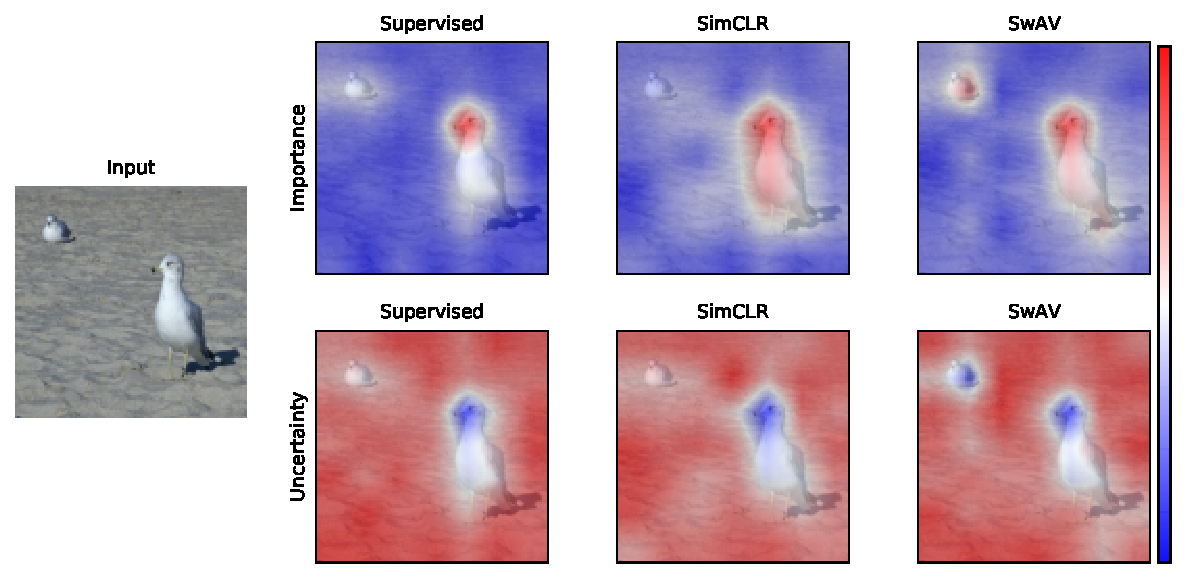
\includegraphics[width=0.47\textwidth]{./images/VOCexample.pdf}
    \caption{RELAX explations and uncertainty estimates for a VOC image.}
    \label{fig:relax}
\end{figure}

\subsubsection{Explaining Representation Learning with Perceptual Components \cite{yarici2024explaining}}
The paper introduces a novel method to analyze representation spaces using three key perceptual components: color, shape, and texture. We employ selective masking of these components to observe changes in representations, resulting in distinct importance maps for each. Here, importance and uncertainty are found using the RELAX method. \\
\\
\textbf{Making strategies for Perceptual Components:}
\vspace{3mm}
\begin{itemize}
    \item \textbf{Color:} Original image is masked with the grayscale version of the image. Masking operation is denoted as:
    \begin{equation*}
        \mathbf{X_{MC}}= (\mathbf{X} \odot \textbf{M}) + (\mathbf{X_{grayscale}} \odot (1-\textbf{M}))
    \end{equation*}
    where $\mathbf{X_{grayscale}}$ is a grayscale transformed input image and $\mathbf{X_{MC}}$ is color masked image.
    \vspace{3mm}
    \item \textbf{Shape:} Information about shape is extracted from the image by using edge detection. Canny edge detection is used to extract the edges of the image. The masked image is denoted as:
    \begin{equation*}
        \mathbf{X_{MS}}= \mathbf{X_{EdgeImage}} \odot \mathbf{M}  
    \end{equation*}
    where $\mathbf{X_{EdgeImage}}$ is the output of edge detection and $\mathbf{X_{MS}}$ is edge masked image.
    \vspace{3mm}
    \item \textbf{Texture:} First input image is transformed to grayscale and then Gaussian blur is used to mask the image. The masked image is denoted as:
    \begin{equation*}
        \mathbf{X_{MT}}=  (\mathbf{X_{grayscale}} \odot \textbf{M}_{t} + (\mathbf{X_{blur}} \odot (1-\textbf{M}_t))) 
    \end{equation*}
    where $\textbf{X}_{grayscale}$ is the grayscale transformation to the input image, $\mathbf{X_{blur}}$ is gaussian blurred grayscale image  and $\textbf{X}_{MT}$ is texture masked image. Here we use the mask with the addition of edge image and normal mask $\textbf{M}_t=\textbf{ M}  \lor \mathbf{X_{EdgeImage}}$ for masking where $\lor$ is logic element wise OR operator between two binary inputs. This masking ensures that the edges are not affected by blur operation. 
\end{itemize}